\section{Sharp gap-free bounds for the filtered mean}\label{sec:gapfree}
Geometric convergence to an eigenspace requires spectral separation. Estimating
an extremal eigenvalue by a filtered mean is a different task: nearby unwanted
eigenvalues contribute little bias even when their probability mass remains
large. We quantify this distinction without assuming a lower bound on the gap.
Throughout this section, $0<a<1$, $t\geq1$, and the target mass is exactly $a$.
All results remain upper bounds when only a lower bound on $a$ is available,
by substituting that lower bound.

\begin{theorem}[Exact two-point bias envelope]\label{thm:envelope}
Let $q$ be a continuous strictly positive response on $[\lambda_0,1]$,
$\lambda_0<1$, and set $R_t(x)=[q(x)/q(\lambda_0)]^{2t}$. Over all finite
spectra with minimum $\lambda_0$ and all normalized input weights with mass
$a$ on that minimum, the largest possible filtered-mean bias is
\begin{equation}\label{eq:envelope}
 \mathcal B_t(q;a,\lambda_0)
 =\max_{\lambda_0\leq x\leq1}
 \frac{(1-a)(x-\lambda_0)R_t(x)}{a+(1-a)R_t(x)}.
\end{equation}
The maximum is attained by a two-eigenvalue spectrum, with weights $a$ and
$1-a$. In particular, this is an exact worst-case envelope for a fixed filter,
not an optimization over filters or a quantum-query lower bound.
\end{theorem}
\begin{proof}
Write the outside weights as $(1-a)\nu_i$, where $\sum_i\nu_i=1$.
If the right side of \eqref{eq:envelope} is $b$, its pointwise definition gives
$(1-a)(x-\lambda_0)R_t(x)\leq b[a+(1-a)R_t(x)]$.
Averaging with $\nu_i$ and dividing by the positive denominator proves the
upper bound. Conversely, put all outside mass on a maximizing $x$.
The maximum is positive for some $x>\lambda_0$, so a maximizing spectrum can
indeed have minimum mass exactly $a$. This is an elementary instance of
linear-fractional extremization \cite{CharnesCooper}; the reduction itself is
not proposed as a new optimization principle.
\end{proof}

For comparison, let $q_{\rm G}(x)=\cos(\beta x)$ and
$q_{\rm D}(x)=\cos(\beta\sqrt{x})$, with $0<\beta<\pi/2$. The latter is the
right-space response of the even cosine transform of a Hermitian dilation.
Define, for $k=1,2$,
\begin{equation}\label{eq:constant}
 A_a=\frac{a}{1-a},\qquad
 C_k(a)=\max_{y\geq0}\frac{y^{1/k}}{1+A_a e^y},\qquad
 y_k=\frac1k+W_0\!\left(\frac{e^{-1/k}}{kA_a}\right).
\end{equation}
Here $W_0$ is the nonnegative real branch of the Lambert function, and the
maximum defining $C_k$ is evaluated at $y_k$.

\begin{theorem}[Uniform rates and sharp leading constants]\label{thm:rates}
Uniformly over $0\leq\lambda_0<1$ and over the finite spectra and weights in
Theorem~\ref{thm:envelope},
\begin{equation}\label{eq:rates}
 \mu_t-\lambda_0\leq
 \begin{cases}
 C_2(a)/(\beta\sqrt{t}), &q=q_{\rm G},\\
 C_1(a)/(\beta^2 t), &q=q_{\rm D}.
 \end{cases}
\end{equation}
For each fixed $a,\beta$, the leading constants and powers of $t$ are
asymptotically attained by two-point spectra with $\lambda_0=0$ and
$x_t=(y_k/(t\beta^2))^{1/k}$, using $k=2$ for G and $k=1$ for D.
The worst-case noiseless errors of the estimator $\alpha\sqrt{\mu_t}$
therefore have rates $t^{-1/4}$ and $t^{-1/2}$, respectively.
These statements concern scalar iterations, with no matched oracle-cost claim.
\end{theorem}
\begin{proof}
Let $h=-\log q$. For the Gram response,
$h'(x)=\beta\tan(\beta x)\geq\beta^2 x$, so, writing $d=x-\lambda_0$,
$2t[h(x)-h(\lambda_0)]\geq t\beta^2(x^2-\lambda_0^2)
\geq t\beta^2d^2$.
For the dilation response, continuous extension at zero gives
$h'(x)=\beta\tan(\beta\sqrt{x})/(2\sqrt{x})\geq\beta^2/2$,
hence the same expression is at least $t\beta^2d$.
The ratio in \eqref{eq:envelope} increases with $R_t$. Substituting
$R_t\leq e^{-t\beta^2d^k}$ and setting $y=t\beta^2d^k$ proves
\eqref{eq:rates}. Differentiating the definition of $C_k$ gives
$(ky-1)e^y=1/A_a$, which has the unique solution \eqref{eq:constant}.
For the matching lower bound, take $\lambda_0=0$ and $x=x_t$. The expansion
$2t\log\cos(\beta x_t^{k/2})=-y_k+O(t^{-1})$ proves that the ratio
of the attained bias to the upper bound tends to one. Finally,
$|\sqrt{\mu_t}-\sqrt{\lambda_0}|\leq\sqrt{\mu_t-\lambda_0}$,
with equality at $\lambda_0=0$.
\end{proof}

\paragraph{Interpretation and limits.}
The extremizing spectrum changes with $t$. These rates are worst-case
statements across spectra, not the asymptotic rate of a fixed gapped matrix.
For any fixed positive minimum, $h'(\lambda_0)>0$ and the same argument gives
$\mathcal B_t\leq C_1(a)/(2t h'(\lambda_0))$ for these two responses.
Conversely, there is no uniform gap-free improvement of target fidelity over
$a$: an outside eigenvalue can approach $\lambda_0$ arbitrarily closely at
each finite $t$. The distinction between mean bias and state fidelity is thus
essential. The zero-minimum examples prove sharpness of the estimator's bias,
not hardness of estimating a minimum already promised to be zero; strictly
positive minima tending sufficiently quickly to zero give the same limiting
constants by continuity.

The success probability still obeys
$a q(\lambda_0)^{2t}\leq Z_t\leq q(\lambda_0)^{2t}$ for these decreasing
responses. At the kernel boundary $Z_t\geq a$; at a fixed positive minimum it
can be exponentially small. Thus a gap-free bias guarantee does not establish
a uniform efficient preparation or estimation algorithm.

\section{Normalization, polynomial baselines, and implementation error}
\label{sec:normalization}
\paragraph{A normalization-induced restart penalty.}
For the Taylor proxy used above, $P_{m_0}(0)=1$ but
$\widetilde P_{m_0}(0)=(1+\delta_{m_0})^{-1}$. A scalar rescaling leaves all
conditional weights unchanged while multiplying the success probability by
$(1+\delta_{m_0})^{-2t}$. For example, with $\beta=1.2$ and $m_0=1$,
$\delta_{m_0}=0.0864$; the penalty factor at $t=128$ is
$6.12\times10^{-10}$. Even on a kernel-bearing input, any fixed positive
global margin destroys the ideal constant success floor as $t$ grows.
Keeping that factor bounded away from zero requires
$t\log(1+\delta_{m_0})=O(1)$. Target normalization is already central to
established polynomial projector constructions \cite{LinTongFilter}; the
observation here identifies its concrete consequence for this Taylor proxy.

\paragraph{Fixed-degree reference responses.}
For $0<\beta<\sqrt{2}$ set $c=\beta^2/2<1$ and consider
\[
 Q_{\rm G}(x)=1-cx^2,\qquad Q_{\rm D}(x)=1-cx.
\]
As polynomials in the normalized singular value $s$, these are $1-cs^4$
and $1-cs^2$, respectively; both are even and bounded between zero and one
on $s\in[-1,1]$, and both preserve the kernel exactly at the response level.
These elementary polynomial filters are comparison baselines, not new
algorithmic primitives. The bounds and sharp constants of
Theorem~\ref{thm:rates} hold for them as well: for $k=2,1$,
$-\log(1-cx^k)$ has derivative at least $ckx^{k-1}$, and its local expansion
gives the same matching lower bound. This shows that the ideal cosine
response is unnecessary for obtaining these scalar rates. No claim of
degree-optimality follows, and compiled QSVT success blocks must realize the
specified normalization; an additional factor per iteration would reintroduce
the restart penalty.

\paragraph{Transfer to an approximate success block.}
Let $C$ and $\widetilde C$ be contractions and
$\|\widetilde C-C\|\leq E$, with $u=C^t\psi$ and $Z_t=\|u\|^2>0$.
Telescoping gives $\|\widetilde C^t\psi-u\|\leq tE$ and
$|\sqrt{\widetilde Z_t}-\sqrt{Z_t}|\leq tE$. If $tE<\sqrt{Z_t}$,
the implemented accepted state exists, its distance in vector norm from the
ideal normalized state is at most $2tE/\sqrt{Z_t}$, and hence
\begin{equation}\label{eq:robust}
 |\widehat\sigma-\sigma_0|
 \leq\alpha\sqrt{\mathcal B_t(q;a,\lambda_0)
                  +2tE/\sqrt{Z_t}+\zeta}
\end{equation}
on the event that Bernoulli readout error is at most $\zeta$.
Indeed, normalization changes the vector error by at most a factor two,
pure-state trace distance is no larger than that vector distance, and the
expectation of $0\leq G\leq I$ changes by at most trace distance.
This is a conditional perturbation estimate, not a new stability principle;
encoding noise, phase synthesis and normalization must all be included in
$E$ before \eqref{eq:robust} is used. At a kernel, $\sqrt{Z_t}\geq\sqrt a$
provides an explicit tolerance; for a positive minimum, conditioning may
make this tolerance exponentially restrictive.

\section{Numerical audit of the sharp bounds}\label{sec:envelope-audit}
The new deterministic script \texttt{experiments/qmsve\_gapfree\_envelope.py}
evaluates the exact one-dimensional envelope and independently checks it
against 1,000 random thirteen-level spectra, with seed 20261027, and dense
20,001-point grids. A stationary-point equation is used for the envelope;
the Lambert expression for $C_k$ is cross-checked by a scalar root equation.
No tested mixture or grid value exceeded its predicted bound by more than
$2\times10^{-12}$. These finite checks support the implementation and do
not replace the proofs. The JSON records versions, base commit, source hash,
parameters, maximizers, and success probabilities.

\begin{figure}[tb]
\centering
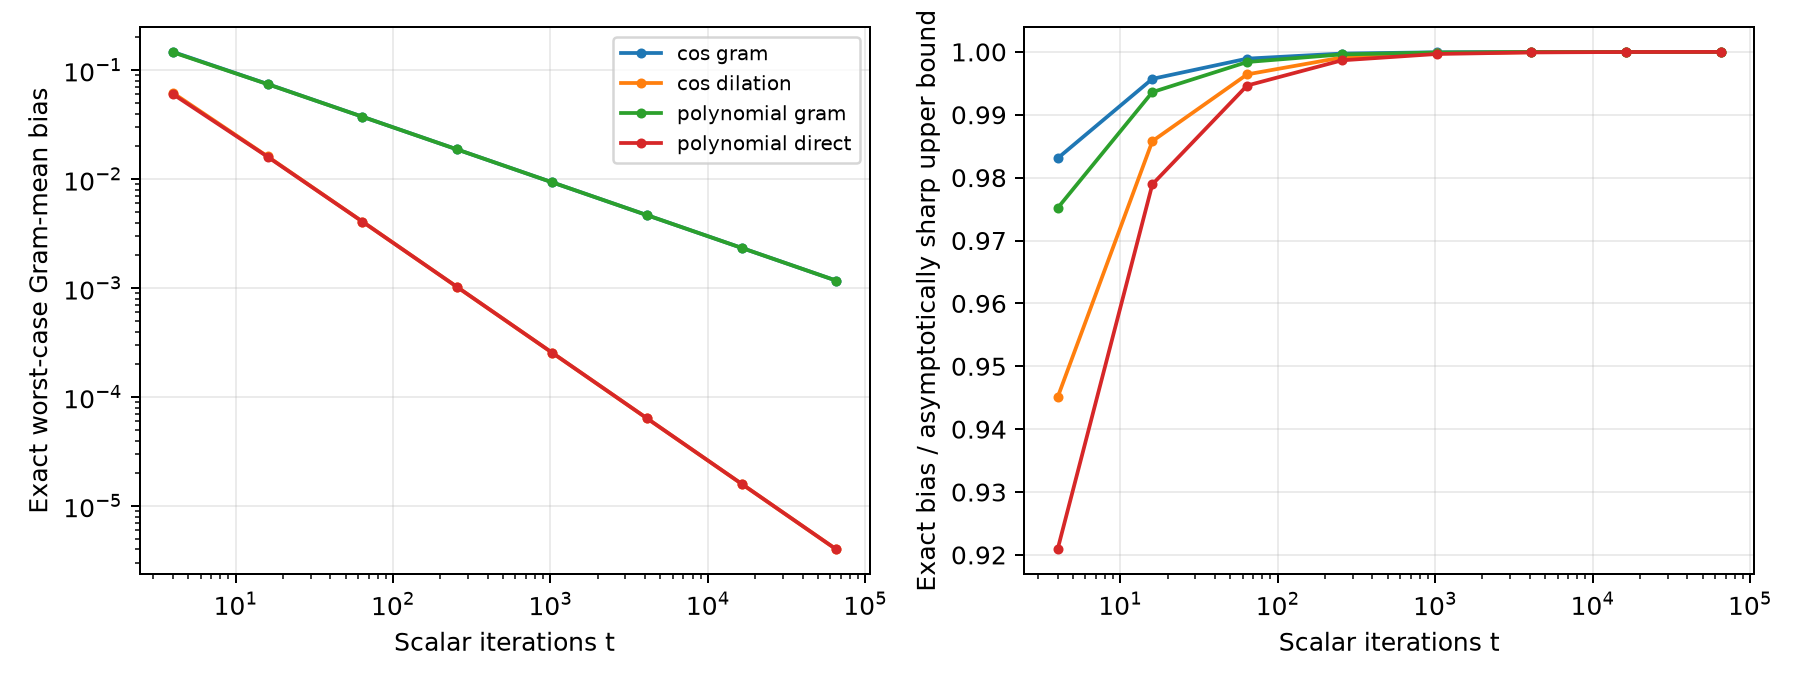
\includegraphics[width=\linewidth]{../../figures/qmsve_gapfree_envelope.png}
\caption{Exact worst-case mean bias at $a=0.4$, $\beta=1.2$, and its ratio
to the sharp asymptotic upper bound. Each point uses its own two-level
adversarial spectrum; it is not a trajectory on one fixed matrix. Scalar
iterations are compared; oracle costs are not matched.}
\label{fig:envelope}
\end{figure}
At $a=0.4$, $C_2(a)=0.360257$ and $C_1(a)=0.378089$. All four responses
reach at least $99.9\%$ of their respective asymptotic bounds by $t=65536$
for the tested overlaps $a=0.1,0.4,0.9$. In the $a=0.4$ polynomial-Gram
extremizer at $t=128$, the kernel-preserving response has success $0.6625$;
the globally scaled degree-two Taylor response has the identical posterior
but success $4.05\times10^{-10}$. This comparison isolates the scaling
penalty and does not compare full circuits.
